\begin{gbox}{{\LARGE !}}{grey1}{{\large \textbf{Multi-Unit Spectroscopy Explorer
      (MUSE)}}}
  \begin{minipage}{\linewidth}
    \begin{wrapfigure}{r}{0pt}
      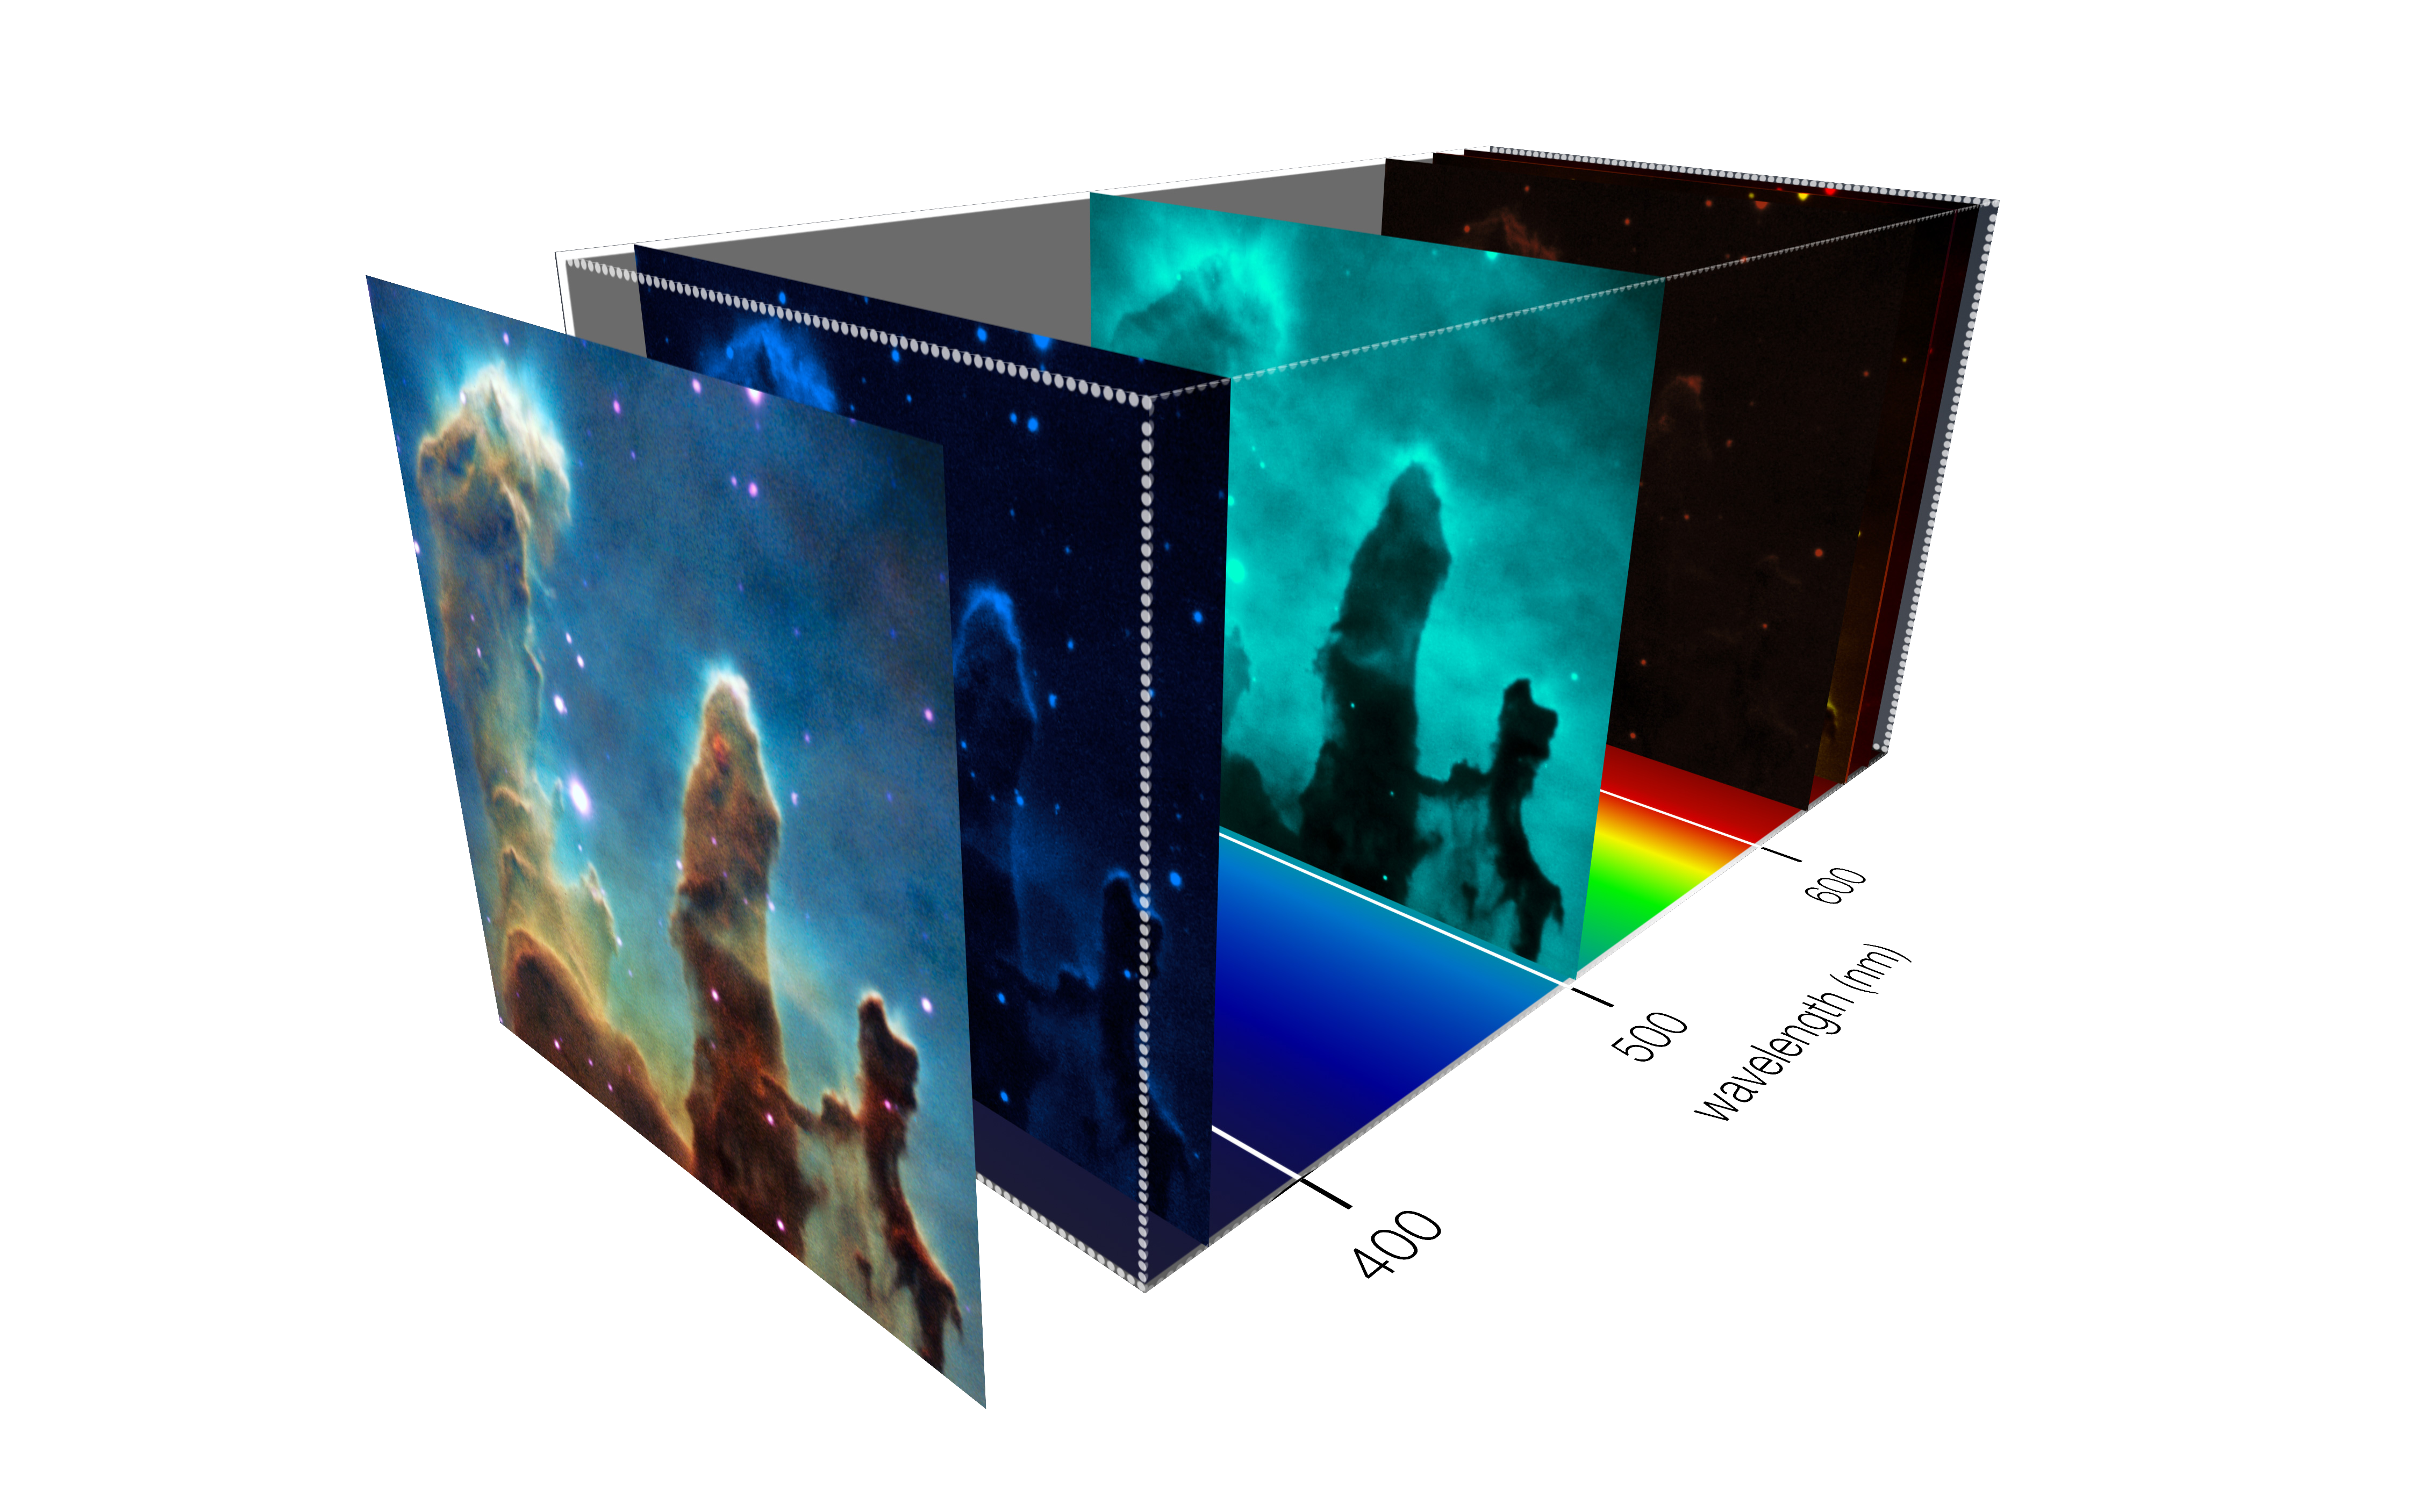
\includegraphics[width=15cm]{MUSE/MUSE.png}
    \end{wrapfigure}
    \strut {\small The Multi Unit Spectroscopic Explorer (MUSE) is a second
      generation instrument installed on the Nasmyth focus of UT4 at the Very
      Large Telescope (VLT) of the European Southern Observatory (ESO). MUSE is
      a powerful spectrograph fed by a new adaptive optics system. it is
      uniquely well suited to the study of faint galaxies in the early Universe
      as well as to objects in our own solar system.}
  \end{minipage}

  \vspace{1cm}

  \begin{minipage}{\linewidth}
    \begin{center}
      \includegraphics[width=0.9\linewidth]{MUSE/logos.png}
    \end{center}
  \end{minipage}
\end{gbox}